Følgende er baseret på \cite[pp. 27-38]{rose2012software}.

I følge Sarasvathy er der to paradigmer indenfor entrepenørskab.
Disse gør sig også gældende indenfor software entrepenørskab.
De to paradigmer, ADE og CDE, agerer poler, på samme måde som traditionel og agil software udvikling.

Det første af de to paradigmer er ADE:\\
\centering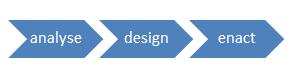
\includegraphics[width=.5\textwidth]{graphics/ade}

ADE minder i høj grad om traditionel software udvikling, idet der forsøges at planlægges og designes således der vil forekomme færre uforudsete problemer.

I modsætning til ADE vil CDA ikke forudsige, men nærmere forsøge at kontrollere.
Dette er en iterativ proces, i stil med agil software udvikling:\\
\centering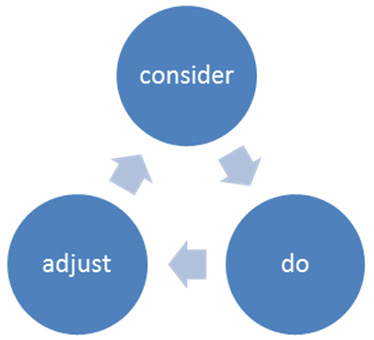
\includegraphics[width=.5\textwidth]{graphics/cda}

Som \citet{rose2012software} nævner vil de fleste organisationer falde under begge paradigmer.
Dette ser vi umiddelbart også som værende tilfældet for vores forretning, hvorfor vi systematisk vil gennemgå sammenligningstabellen i \citet[p. 38]{rose2012software}.

\paragraph{Process:} Primært sekventiel, vi har hardware samt meget sikkerhedskritisk software, så det kunne være katastrofalt at få rullet et usikkert produkt ud for hurtigt.

\paragraph{Understanding of future:} Vi vil gerne styre fremtiden, altså sætte en høj standard for sikkerhed som andre vil få svært ved at følge.
Usability og at det passer ind i kundens/brugernes proces er vigtigt, så her skal vi være gode til at tilpasse os så vi kan få solgt vores produkt, altså så folk ikke ser det som en for stor hindring.

\paragraph{Attitude to market:} Forsøg på at skabe et nyt marked, ved at bringe noget som folk ikke er klar over de har brug for.
Selvom det som sådan ikke er et nyt produkt.

\paragraph{Attitude to technology development:} Vi vil gerne være foran de andre så vi kan sætte standarden for hvad god sikkerhed, så vi er de eneste der kan levere det optimalt.

\paragraph{Role of business planning:} Vi har ikke råd til fejl her, da vist vi først får leveret en dårlig løsning, vil folk få svært ved at have tillid til os efterfølgende.

\paragraph{Software development:} Agile og lean, da vi gerne vil have et velafprøvet og veltestet produkt.
Usability er igen vigtigt, da vi gerne vil have vores produkt så seamless integreret som muligt.

\paragraph{Attitude to change:} Nyt marked, så vi ser ændringer som muligheder for at lave et bedre og mere fleksibelt produkt.

\paragraph{Funding approach:} Venture capital så vi kan få sikret kvalitet inden produktet frigives, sådan at vi ikke mister credibility ved en for dårlig tidlig løsning.

\paragraph{Approach to others working in the same areas:} Samarbejde er godt.
Hvis vi kan undgå at opfinde/lave alting selv er det en fordel.
Så kan vi udnytte andres erfaringer, merge idéer og sælge dem videre som pakkeløsning.

\paragraph{Approach to intellectual property:} Platformen er lukket, men de enkelte dele er åbne.

\paragraph{Partnering and Networking:} Netværk og samarbejde er godt, samme som ovenover.

\paragraph{Time to market:} Se `Funding approach'.

\paragraph{Phases or activities in the business model process}

\subparagraph{Mobilize}
\begin{itemize}
\item Test preliminary business ideas (Diskuter internt, cross functional/tier)
\item Assemble team (Relater Resource-based (husk usability-gut) og value-chain)
\end{itemize}

\subparagraph{Understanding}
\begin{itemize}
\item Study potential customers (Undersøg nuværende arbejdsprocesser og sikkerhedsprotokoller, hvordan de håndterer passwords, hos potentielle kunders virksomhed)
\item Interview experts (Interview René Rydhof, Kramshøj, Jacob Nielsen)
\item Research already tried (Nuværende relaterede firmaer og deres produkter)
\end{itemize}

\subparagraph{Design}
\begin{itemize}
\item Prototype setup inhouse (2 rum med kort-indgang og computere hvor passwords kan bruges)
\item Brainstormet og testet BMs (Venture Capital og Ivan)
\end{itemize}

\subparagraph{Implement}
\begin{itemize}
  \item Communicate and involve (Alle i vores virksomhed skal være med på den)
\end{itemize}

\subparagraph{Manage}
\begin{itemize}
  \item Se ovenover: Attitude to change, technology development, understanding future
\end{itemize}

\todo{Oste-bogen, side 244-?}
